\documentclass[11pt]{article}
\newcommand{\coursedocname}{Problem Set 3}

\usepackage[utf8]{inputenc}
\usepackage[T1]{fontenc}
\usepackage{lmodern}
\usepackage[margin=1in]{geometry}
\usepackage[dvipsnames]{xcolor}
\usepackage{graphicx, booktabs, enumitem, float, framed, caption, multirow}
\usepackage{fancyhdr}
\usepackage{tcolorbox}
\usepackage{listings}
\usepackage{tikz}
\usepackage{setspace}
\usepackage{needspace}
\IfFileExists{algorithm.sty}{%
  \usepackage{algorithm}
  \usepackage[noend]{algpseudocode}
  \newcommand{\hasalgorithms}{}%
}{}
\usepackage{amsmath,amssymb,bm,xcolor}





\newcommand{\cellbelief}{B}            %

\usepackage{hyperref}

\definecolor{DartmouthGreen}{HTML}{00693E}
\newcommand{\dgreen}[1]{\textcolor{DartmouthGreen}{#1}}
\newcommand{\dgbf}[1]{\textbf{\dgreen{#1}}}      %
\urlstyle{same}
\hypersetup{
    colorlinks=true,
    linkcolor=DartmouthGreen,
    filecolor=DartmouthGreen,
    citecolor=DartmouthGreen,
    urlcolor=DartmouthGreen,
    breaklinks=true
}

\newcommand{\coursenumber}{COSC 81/281}
\newcommand{\courseterm}{Fall 2026}
\newcommand{\gradescopelink}{\textbf{Gradescope} (\url{https://www.gradescope.com/courses/1372528})}

\newcommand{\psThreeDue}{Tuesday, October 20 (11:59pm ET)}

\setlength{\parindent}{0pt}
\setlength{\parskip}{6pt plus 2pt minus 1pt}
\setlength{\headheight}{13.6pt}
\setlength{\emergencystretch}{3em}
\providecommand{\tightlist}{\setlength{\itemsep}{0pt}\setlength{\parskip}{0pt}}
\setcounter{secnumdepth}{0}

\DeclareRobustCommand{\callout}[2][gray!10]{%
  \begin{tcolorbox}[left=8pt, arc=0pt, outer arc=0pt,
                    colframe=#1, colback=#1, coltext=black]#2\end{tcolorbox}}




\newcommand{\gradstar}{$\bigstar$~\textsf{\small (required for 281; optional for 81)}~}
\newcommand{\bonusq}{\textsf{\small\textbf{[Bonus]}}~}
\newcommand{\bonus}{\bonusq}

\newcommand{\setupheader}[1]{%
  \fancypagestyle{default}{%
      \lhead{#1}
      \chead{}
      \rhead{\textbf{\coursenumber}}
      \lfoot{}
      \cfoot{}
      \rfoot{\thepage}
      \renewcommand{\headrulewidth}{0.4pt}
      \renewcommand{\footrulewidth}{0.4pt}
  }
  \pagestyle{default}
  \fancypagestyle{plain}{\pagestyle{default}}
}
\newcommand{\setupexamheader}[1]{%
  \fancypagestyle{default}{%
      \lhead{#1}
      \chead{Name:}
      \rhead{}
      \lfoot{}
      \cfoot{}
      \rfoot{\thepage}
      \renewcommand{\headrulewidth}{0.4pt}
      \renewcommand{\footrulewidth}{0.4pt}
  }
  \pagestyle{default}
  \fancypagestyle{plain}{\pagestyle{default}}
}
\newcommand{\pstitle}[2]{%
  \title{\textbf{\coursenumber:} #1}
  \author{\textbf{Due} #2\\
  }
  \date{}
}

\newcommand{\coursenotice}{%
  \callout{Problem sets are graded \textbf{pass/fail on completion}, and
  there are no late days. The problem sets are where the learning happens,
  and they are the best available practice for the midterm and final exam.
  Submit to \gradescopelink\ and assign each question to a page in your
  submission. Questions are welcome on \dgbf{Slack}. Starred ($\bigstar$)
  questions are required for COSC 281 students and optional (ungraded) for
  COSC 81 students.}}

\lstset{
  language=python,
  basicstyle=\ttfamily,
  commentstyle=\color{BrickRed},
  stringstyle=\color{ForestGreen},
  showstringspaces=false,
  breaklines=true,
  breakatwhitespace=true,
  keywordstyle=\color{Purple},
  emph={def},
  emphstyle=\color{RoyalBlue}
}
\lstnewenvironment{itemlisting}[1][]
 {\mbox{}\vspace*{-\baselineskip}%
  \lstset{xleftmargin=\leftmargin, linewidth=\linewidth, #1}}
 {}

\makeatletter
\def\fps@figure{htbp}
\makeatother
\ifdefined\hasalgorithms
\fi

\newcommand{\docfooter}{\vfill\begin{tiny}Updated \today\end{tiny}}

\newenvironment{studentanswer}[1]
  {\par\medskip\noindent
   \begin{tcolorbox}[height from=#1 to 100cm, colback=white, colframe=gray!60,
     boxrule=0.6pt, arc=0pt, outer arc=0pt, left=7pt, right=7pt,
     top=7pt, bottom=7pt, title={Answer / work}, fonttitle=\small,
     coltitle=black, colbacktitle=gray!8, titlerule=0pt]
   \ignorespaces}
  {\end{tcolorbox}\par}

\setupheader{\coursenumber\ -- \courseterm\ -- \coursedocname}
\pstitle{Problem Set 3: Estimation and Control}{\psThreeDue}

\begin{document}
\maketitle
\coursenotice
\begin{quote}\small\textbf{AI Policy.} You may use any AI tools you like to assist you with your assignments, and you should, as that is likely how you will work for the rest of your career.
That being said, the written portions are practice for the in-class midterm and exam, which are closed book and on paper. You should strive to answer these yourself and use AI as a tutor and not an oracle.
\end{quote}

\callout{Please include an AI Tool Disclosure Below \vspace{50pt}}

\raggedbottom
\Needspace{8cm}
\textbf{What to submit.} Submit to \gradescopelink:\vspace{-10pt}
\begin{enumerate}\tightlist
\item \textbf{Written work (PDF)}: your answers to Part 1 and every figure
      and short analysis requested in Part 2. You may write on this handout or use
      \texttt{ps3/handout.tex}. Put each answer or figure in the
      corresponding \texttt{studentanswer} environment, after this marker:
      \begin{center}
      \texttt{\%\%\%\%\% SOLUTION HERE \%\%\%\%\%}
      \end{center}
      Then compile the file. Assign each question to its page or pages when you upload. You may add
      pages for longer answers or figures; typed response boxes expand as needed.
\item \textbf{Code}: \texttt{particle\_filter.py} and
      \texttt{control\_gains.py}. Before submission, run the public autograder from
      the repository root:
      \begin{center}\texttt{python ps3/code/autograder.py}\end{center}
\end{enumerate}

\clearpage
\section{Part 1: Written problems}

Show your work in the response area for each part. These problems can be
answered from the information provided, without running the programming
tasks. You may use the programming results as supporting evidence where
requested.

\subsection*{P1: A corridor as a hidden Markov model}
A robot occupies one of three cells, numbered from left to right. Only
cell 3 has a door. Let $X_t$ be its cell and $Z_t$ its binary sensor
reading, either \texttt{door} or \texttt{no door}. Initially $X_0$ is
uniform. The sensor has
\[
P(Z_t=\texttt{door}\mid X_t=3)=0.9,\qquad
P(Z_t=\texttt{door}\mid X_t\ne3)=0.3.
\]
When commanded to move right from cell 1 or 2, the robot succeeds with
probability $1/2$ and otherwise stays. In cell 3 it stays with probability 1.
The robot receives one rightward command, then takes its first sensor
reading at time 1. That reading is \texttt{door}.

Let $x_i$ denote cell $i$, and write $\cellbelief(x_i)$ for its belief
probability at the stage being computed. Initially,
$\cellbelief(x_i)=1/3$ for each of the three cells.
Compute this filtering update in three stages. In each response grid,
write one value in each cell, including any zeros. Each value describes
the probability or weight assigned to that cell, not a particular
robot trajectory. Show your calculations below the grid and leave
your results as fractions.
\begin{center}
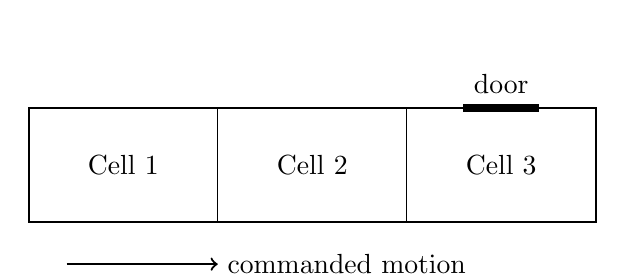
\begin{tikzpicture}[scale=1.2]
\draw[thick] (0,0) rectangle (6,1.2);
\draw (2,0)--(2,1.2); \draw (4,0)--(4,1.2);
\node at (1,.6) {Cell 1}; \node at (3,.6) {Cell 2};
\node at (5,.6) {Cell 3};
\draw[line width=3pt] (4.6,1.2)--(5.4,1.2);
\node[above] at (5,1.25) {door};
\draw[->,thick] (.4,-.45)--(2,-.45);
\node[right] at (2,-.45) {commanded motion};
\end{tikzpicture}
\end{center}
\begin{enumerate}[label=(\alph*)]
\item \begin{minipage}[t]{\linewidth} Compute the belief after the rightward command using
\textbf{only the motion model}. Do not use the \texttt{door} reading or
any sensor likelihoods in this part. Fill the grid with the predicted
belief $\cellbelief(x_i)=P(X_1=x_i)$ for $i=1,2,3$. Show the contributions
from all previous cells that can reach each destination cell.

\begin{studentanswer}{5cm}
%%%%% SOLUTION HERE %%%%%
\begin{center}
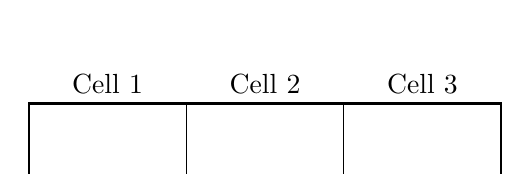
\begin{tikzpicture}
\draw[thick] (0,0) rectangle (6,1);
\draw (2,0)--(2,1); \draw (4,0)--(4,1);
\foreach \x in {1,2,3}{\node[above] at (2*\x-1,1){Cell \x};}
\end{tikzpicture}
\end{center}
\end{studentanswer}

\end{minipage}
\end{enumerate}

\clearpage
\noindent\textbf{P1 (continued)}
\begin{enumerate}[label=(\alph*),start=2]
\item \begin{minipage}[t]{\linewidth} Now incorporate the \texttt{door} reading. Multiply each predicted
cell probability from part (a) by the likelihood of this reading in
that cell. Fill the grid with these three unnormalized weights. Do not
normalize them yet.

\begin{studentanswer}{4cm}
%%%%% SOLUTION HERE %%%%%
\begin{center}
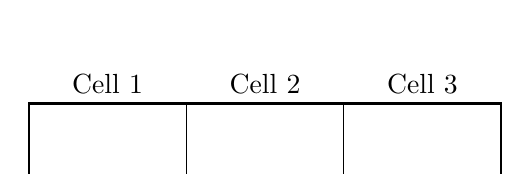
\begin{tikzpicture}
\draw[thick] (0,0) rectangle (6,1);
\draw (2,0)--(2,1); \draw (4,0)--(4,1);
\foreach \x in {1,2,3}{\node[above] at (2*\x-1,1){Cell \x};}
\end{tikzpicture}
\end{center}
\end{studentanswer}

\end{minipage}

\item \begin{minipage}[t]{\linewidth} Apply Bayes' rule by summing the weights from part (b), then dividing each weight by that
sum. Fill the grid with the resulting belief
$\cellbelief(x_i)=P(X_1=x_i\mid Z_1=\texttt{door})$. Check that its three entries
sum to one. Briefly explain why the sensor likelihood $0.9$ is not
itself the updated probability that the robot is in cell 3.

\begin{studentanswer}{5cm}
%%%%% SOLUTION HERE %%%%%
\begin{center}
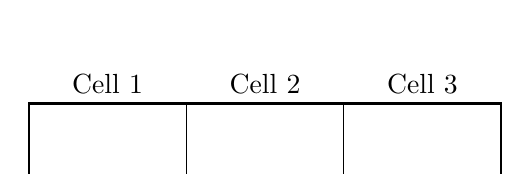
\begin{tikzpicture}
\draw[thick] (0,0) rectangle (6,1);
\draw (2,0)--(2,1); \draw (4,0)--(4,1);
\foreach \x in {1,2,3}{\node[above] at (2*\x-1,1){Cell \x};}
\end{tikzpicture}
\end{center}
\end{studentanswer}

\end{minipage}

\end{enumerate}

\clearpage
\subsection*{P2: Moving and weighting particles on a grid}
Six equally weighted particles represent possible robot locations.
Their coordinates are cell indices $(x,y)$, and each initially has
weight $1/6$. The grid has reflecting left and right boundaries.
For this single prediction, command every particle to move one cell
in the positive $x$ direction. A particle in column 4 instead moves one
cell left to column 3. Its row does not change. There is no motion noise.
\begin{center}
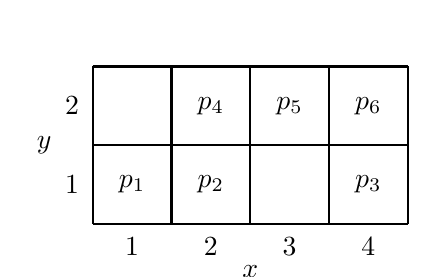
\begin{tikzpicture}[scale=1.0]
\draw[step=1,thick] (0,0) grid (4,2);
\foreach \x in {1,2,3,4}{\node[below] at (\x-.5,-.05){$\x$};}
\foreach \y in {1,2}{\node[left] at (-.05,\y-.5){$\y$};}
\node[below] at (2,-.4){$x$}; \node[left] at (-.4,1){$y$};

\node at (.5,.5){$p_1$}; \node at (1.5,.5){$p_2$};
\node at (3.5,.5){$p_3$}; \node at (1.5,1.5){$p_4$};
\node at (2.5,1.5){$p_5$}; \node at (3.5,1.5){$p_6$};
\end{tikzpicture}
\end{center}
\begin{enumerate}[label=(\alph*)]
\item \begin{minipage}[t]{\linewidth} Draw the particle labels in their cells after the motion. More than
one particle may occupy a cell.

\begin{studentanswer}{4cm}
%%%%% SOLUTION HERE %%%%%
\begin{center}
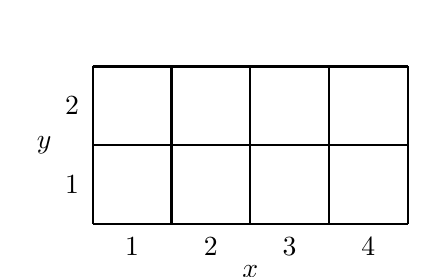
\begin{tikzpicture}[scale=1.0]
\draw[step=1,thick] (0,0) grid (4,2);
\foreach \x in {1,2,3,4}{\node[below] at (\x-.5,-.05){$\x$};}
\foreach \y in {1,2}{\node[left] at (-.05,\y-.5){$\y$};}
\node[below] at (2,-.4){$x$}; \node[left] at (-.4,1){$y$};
\end{tikzpicture}\end{center}
\end{studentanswer}

\end{minipage}
\end{enumerate}
\clearpage
\noindent\textbf{P2 (continued)}

The sensor now reports \texttt{bright}. The table gives the likelihood of
that reading at each possible cell, $P(\texttt{bright}\mid x,y)$.
These are probabilities of a reading given a location, not probabilities
of locations.
\begin{center}
\begin{tabular}{c|cccc}
 & $x=1$ & $x=2$ & $x=3$ & $x=4$\\ \hline
$y=2$ & $1/4$ & $1/2$ & $3/4$ & $1/2$\\
$y=1$ & $1/4$ & $1/4$ & $1/2$ & $3/4$
\end{tabular}
\end{center}
For correction, multiply each particle's previous weight by the
likelihood in its new cell. The unnormalized weight of a cell is the
sum of these products for every particle in that cell. Empty cells
have weight zero.
\begin{enumerate}[label=(\alph*),start=2]
\item \begin{minipage}[t]{\linewidth} Fill every cell of the grid below with its unnormalized weight
after the \texttt{bright} reading. Add the contributions of all particles
in that cell, and write zero in cells containing no particles. Show how
you account for cells containing more than one particle.

\begin{studentanswer}{5.5cm}
%%%%% SOLUTION HERE %%%%%
\begin{center}
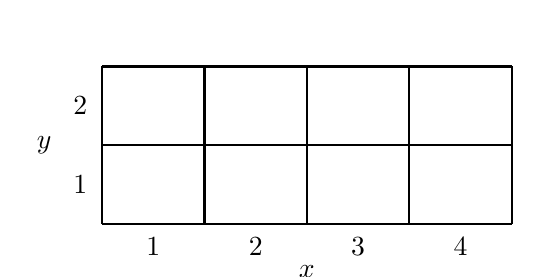
\begin{tikzpicture}[x=1.3cm,y=1cm]
\draw[step=1,thick] (0,0) grid (4,2);
\foreach \x in {1,2,3,4}{\node[below] at (\x-.5,-.05){$\x$};}
\foreach \y in {1,2}{\node[left] at (-.05,\y-.5){$\y$};}
\node[below] at (2,-.4){$x$}; \node[left] at (-.4,1){$y$};
\end{tikzpicture}
\end{center}
\end{studentanswer}

\end{minipage}
\item \begin{minipage}[t]{\linewidth} Sum the unnormalized weights from part (b), then divide each cell's
weight by that sum. Fill every cell of the grid below with its normalized
probability, including zeros. Leave all nonzero entries as fractions
and check that the eight cell probabilities sum to one.

\begin{studentanswer}{5.5cm}
%%%%% SOLUTION HERE %%%%%
\begin{center}
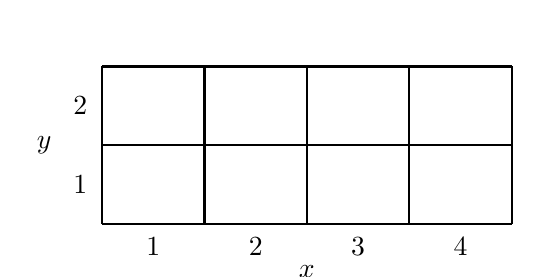
\begin{tikzpicture}[x=1.3cm,y=1cm]
\draw[step=1,thick] (0,0) grid (4,2);
\foreach \x in {1,2,3,4}{\node[below] at (\x-.5,-.05){$\x$};}
\foreach \y in {1,2}{\node[left] at (-.05,\y-.5){$\y$};}
\node[below] at (2,-.4){$x$}; \node[left] at (-.4,1){$y$};
\end{tikzpicture}
\end{center}
\end{studentanswer}

\end{minipage}
\end{enumerate}

\clearpage
\noindent\textbf{P2 (continued)}

For this question, assume the default implementation in which resampling
draws only from the existing particles according to their normalized
weights. Every new particle must be a copy at a cell that already contains
a particle. No samples are drawn from other cells. Each selected copy's
weight is reset to $1/6$. The number of copies at a location is random.
No numerical resampling draw is required here.
\begin{enumerate}[label=(\alph*),start=4]
\item \begin{minipage}[t]{\linewidth} \gradstar Suppose the robot's true location is in a cell that has
no particles after part (a). Can repeated correction and resampling,
without motion or introducing new particle locations, recover that cell?
Explain in two or three sentences.

\begin{studentanswer}{3cm}
%%%%% SOLUTION HERE %%%%%
\end{studentanswer}

\end{minipage}
\end{enumerate}

\clearpage
\subsection*{P3: Building and correcting a map}
A robot uses range measurements to build a map while moving through a
building. Its sensors measure surfaces relative to its current pose.
Answer the following questions without deriving a mapping or SLAM algorithm.
\begin{enumerate}[label=(\alph*)]
\item \begin{minipage}[t]{\linewidth} In localization the map is known, and in mapping with known poses
the robot's locations are supplied. What must a SLAM system estimate
when neither is known?

\begin{studentanswer}{2.5cm}
%%%%% SOLUTION HERE %%%%%
\end{studentanswer}

\end{minipage}
\item \begin{minipage}[t]{\linewidth} Why can an error in the robot's estimated pose distort its current
map? Give one concrete example.

\begin{studentanswer}{3cm}
%%%%% SOLUTION HERE %%%%%
\end{studentanswer}

\end{minipage}
\item \begin{minipage}[t]{\linewidth} The robot recognizes a place it visited earlier. How can a valid
loop closure help, and what could go wrong if the place match is false?

\begin{studentanswer}{3cm}
%%%%% SOLUTION HERE %%%%%
\end{studentanswer}

\end{minipage}
\end{enumerate}

\clearpage
\subsection*{P4: Interpreting planning and estimation results}
Consider the following two independent scenarios. Answer each part in
\textbf{two sentences}. Multiple answers may be acceptable when supported
by the information provided. No implementation or derivation is required.
\begin{enumerate}[label=(\alph*)]
\item \begin{minipage}[t]{\linewidth} A warehouse robot must move between two rooms through a narrow
doorway. Its position and map are known exactly, and it translates without
rotating. The figure shows configuration space, with the robot's footprint
already accounted for in the shaded collision regions.

A grid cell is usable only if its \emph{entire area} is collision-free.
A* connects usable cells sharing a side and reports no path from $S$ to
$G$ on the grid shown. An RRT using the same geometry returns a route
between these positions, and every connecting motion has been checked
for collision.
\begin{center}
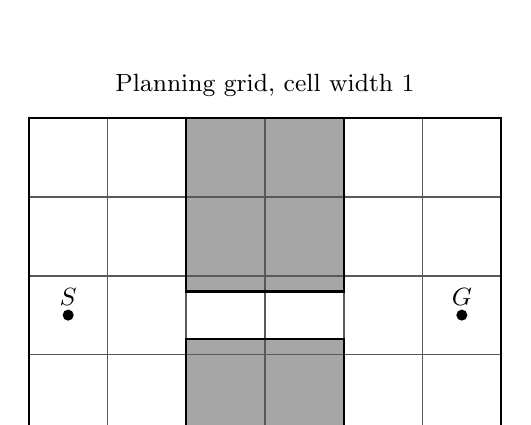
\begin{tikzpicture}[x=1cm,y=1cm,font=\small]
\fill[black!35] (2,0) rectangle (4,1.2);
\fill[black!35] (2,1.8) rectangle (4,4);
\draw[step=1,black!65,line width=.6pt] (0,0) grid (6,4);
\draw[thick] (0,0) rectangle (6,4);
\draw[thick] (2,0)--(2,1.2)--(4,1.2)--(4,0);
\draw[thick] (2,4)--(2,1.8)--(4,1.8)--(4,4);
\fill (.5,1.5) circle(2pt) node[above]{$S$};
\fill (5.5,1.5) circle(2pt) node[above]{$G$};
\node[above] at (3,4.15){Planning grid, cell width 1};
\end{tikzpicture}

\small Shading marks configurations in collision.
The outer rectangle bounds the planning region.
\end{center}
Explain how the two planning results can both be correct. Propose one
change to the A* planning setup that could recover a route, and identify
a computational cost of that change.

\begin{studentanswer}{4cm}
%%%%% SOLUTION HERE %%%%%
\end{studentanswer}

\end{minipage}
\end{enumerate}
\clearpage
\noindent\textbf{P4 (continued)}
\begin{enumerate}[label=(\alph*),start=2]
\item \begin{minipage}[t]{\linewidth} A laboratory robot starts with a reasonably accurate position
estimate and follows a marked route. It records wheel odometry and noisy
range measurements. Its motion and measurement models are mildly nonlinear.
The team runs an EKF and a particle filter with 50 particles on the same
recorded inputs, using the same models and initial uncertainty.
The figure illustrates their estimates of one position coordinate.
It does not show the robot's true position.
\begin{center}
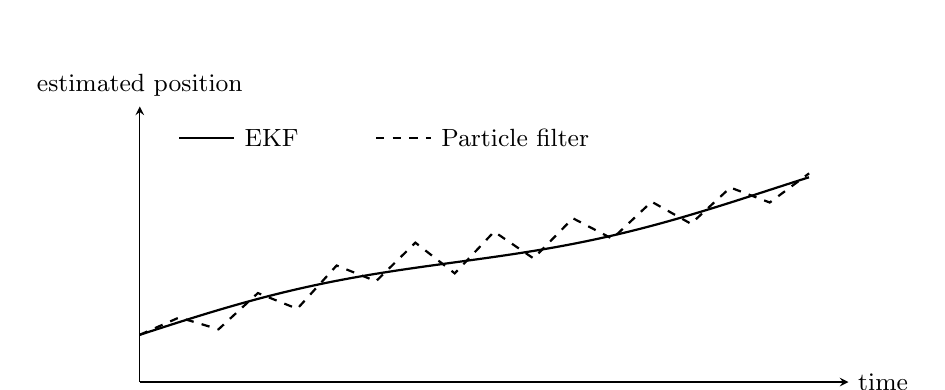
\begin{tikzpicture}[x=1cm,y=1cm,>=stealth,font=\small]
\draw[->] (0,0)--(9,0) node[right]{time};
\draw[->] (0,0)--(0,3.5) node[above]{estimated position};
\draw[thick,domain=0:8.5,samples=100]
 plot (\x,{.6+.23*\x+.12*sin(45*\x)});
\draw[thick,dashed] plot coordinates {
(0,.6) (.5,.82) (1,.67) (1.5,1.13) (2,.93) (2.5,1.48)
(3,1.28) (3.5,1.77) (4,1.38) (4.5,1.91) (5,1.57)
(5.5,2.08) (6,1.82) (6.5,2.29) (7,2.01) (7.5,2.47)
(8,2.28) (8.5,2.65)};
\draw[thick] (.5,3.1)--(1.2,3.1) node[right]{EKF};
\draw[thick,dashed] (3,3.1)--(3.7,3.1) node[right]{Particle filter};
\end{tikzpicture}

\small Illustrative estimates, not measured performance data.
\end{center}
A teammate concludes that the EKF is more accurate because its estimate
is smoother. Assess that conclusion, give one possible explanation for
the difference between the traces, and propose one controlled comparison
that would help the team choose an estimator. Answer in two sentences.

\begin{studentanswer}{4cm}
%%%%% SOLUTION HERE %%%%%
\end{studentanswer}

\end{minipage}

\end{enumerate}

\clearpage
\subsection*{P5: Choosing an estimator}
A robot's estimator has a budget of 1 ms per update. Its particle filter
costs $2\,\mu\mathrm{s}$ per particle, an EKF costs 0.05 ms, and a UKF
costs 0.12 ms. During ordinary tracking the robot's position is
concentrated near one location, and the motion and measurement models
are moderately nonlinear. After an unobserved relocation, two distant
poses can explain the sensor reading.
\begin{enumerate}[label=(\alph*)]
\item \begin{minipage}[t]{\linewidth} How many particles fit within the budget? Explain why a particle
filter could be a good or poor choice for these situations.

\begin{studentanswer}{4cm}
%%%%% SOLUTION HERE %%%%%
\end{studentanswer}

\end{minipage}
\item \begin{minipage}[t]{\linewidth} Explain why an EKF could be a good or poor choice for ordinary tracking
and for the ambiguous relocation. Would Gaussian process and sensor
noise make its belief exact despite the nonlinear models? Explain.
No equations or derivations are required.

\begin{studentanswer}{4cm}
%%%%% SOLUTION HERE %%%%%
\end{studentanswer}

\end{minipage}
\item \begin{minipage}[t]{\linewidth} Explain why a UKF could be a good or poor choice. The UKF can sometimes approximate nonlinear effects better than an
EKF. Is that sufficient to address both situations described above?

\begin{studentanswer}{4cm}
%%%%% SOLUTION HERE %%%%%
\end{studentanswer}

\end{minipage}
\end{enumerate}
\clearpage
\noindent\textbf{P5 (continued)}
\begin{enumerate}[label=(\alph*),start=4]
\item \begin{minipage}[t]{\linewidth} \gradstar Compare how an EKF and a UKF account for a nonlinear motion
or measurement model. What does the UKF use instead of the EKF's local
derivatives? No calculations are required.

\begin{studentanswer}{4cm}
%%%%% SOLUTION HERE %%%%%
\end{studentanswer}

\end{minipage}
\end{enumerate}


\clearpage
\section{Part 2: Programming}

\subsection{Task 1: Particle-filter localization}

Run \texttt{python ps3/code/run\_localization.py} from the repository root
after implementing the three methods in \texttt{particle\_filter.py}.
The driver evaluates localization in the \texttt{corridor} world.

\begin{itemize}
\item \texttt{predict(odom)}: propagate every particle through the provided
      motion model with the commanded relative motion and sampled noise. Use the provided \texttt{motion\_model.sample} and preserve the weights.
\item \texttt{correct(scan)}: reweight particles by the measurement
      likelihood. The starter's sensor model is a likelihood field
      precomputed in the \texttt{Map} class: it returns a log-likelihood per
      particle in one vectorized call. Multiply the previous weights by
      the likelihoods and normalize. Subtract the maximum log-likelihood
      before exponentiating to reduce numerical underflow.
\item \texttt{resample()}: replace the current particles with randomly
      selected copies, with selection probability determined by their
      normalized weights. Copies at likely locations receive more of
      the particle population on average. Reset all weights to $1/N$.
      The systematic procedure below implements this without making
      $N$ independent random draws.
\end{itemize}

\textbf{How to resample.} Number the particles from $0$ to $N-1$ in their
array order. Form cumulative weights
$c_j=w_0+\cdots+w_j$ with \texttt{np.cumsum}. These are the right
endpoints of adjacent intervals covering $[0,1)$, with each interval's
length equal to its particle's weight. Draw one offset $u_0$ uniformly
from $[0,1/N)$ using \texttt{self.rng}, then place $N$ evenly spaced
selection points $u_i=u_0+i/N$. For each point, copy the first particle
$j$ with $c_j>u_i$. The strict inequality assigns a point exactly on an
interval boundary to the interval on its right.

For example, weights $(0.2,0.5,0.3)$ give cumulative weights
$(0.2,0.7,1.0)$. A point at $0.1$ selects particle 0, a point at $0.2$
selects particle 1, and a point at $0.8$ selects particle 2.
\texttt{np.searchsorted(cumulative, points, side="right")} implements
this lookup. Set the last cumulative entry to $1.0$ to avoid a
floating-point roundoff gap. Copy the selected rows into the new
particle array and assign every new weight $1/N$.
When \texttt{u0} is supplied to the method, use that offset directly;
otherwise draw it. Use only \texttt{self.rng} for randomness.

\clearpage
\noindent\textbf{Task 1 (continued)}
\begin{center}
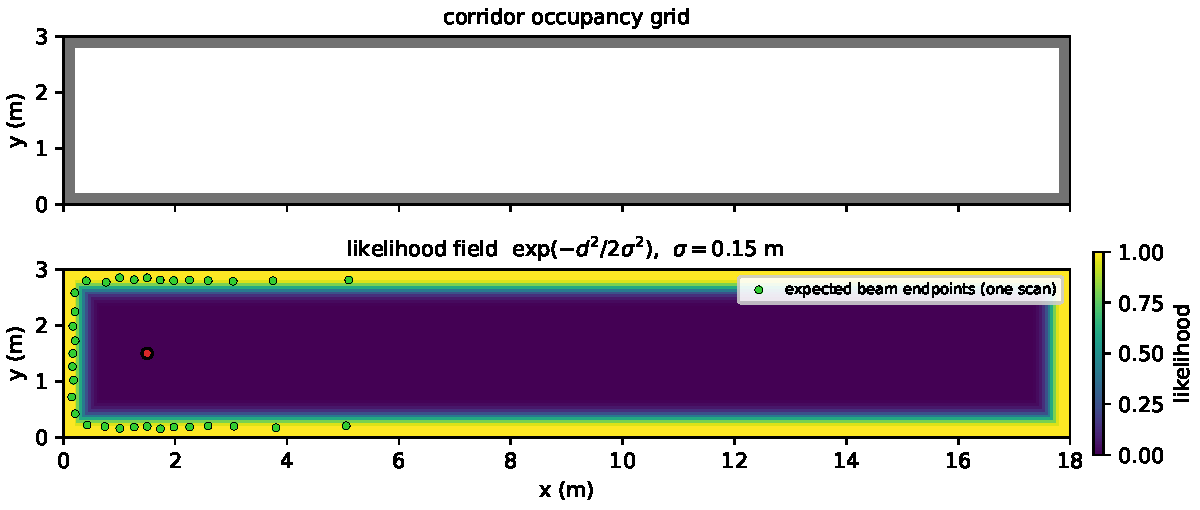
\includegraphics[width=0.68\linewidth]{ps3/figures/likelihood_field.pdf}
\captionof{figure}{The provided sensor model. Top: the \texttt{corridor}
occupancy grid. Bottom: its precomputed likelihood field; bright cells are
near obstacles, so beam endpoints landing there are likely. Green dots are
one scan's expected endpoints from the start pose (red). Your
\texttt{correct} step scores each particle's expected beam endpoints
against this field.}
\end{center}

The simulator's \texttt{ground\_truth\_pose} exists for plotting and
grading only. Do not use it in the estimator.

\textbf{PDF deliverable.} \texttt{ps3\_localization.png}: position error of
your filter's estimate versus time on \texttt{corridor} with 500 particles,
seed 478, produced by the provided plotting call in
\texttt{run\_localization.py}. The autograder also re-runs your filter on
held-out seeds, to check behavior beyond the displayed run.

\textbf{Submission.} Submit the three filter methods in
\texttt{particle\_filter.py}. Include the localization figure in your PDF.

\Needspace{6\baselineskip}
\textbf{PDF responses.}
\begin{enumerate}[label=(\alph*)]

\item \begin{minipage}[t]{\linewidth}
Include \texttt{ps3\_localization.png} from the specified 500-particle run.

\begin{studentanswer}{7cm}
%%%%% SOLUTION HERE %%%%%

\end{studentanswer}

\end{minipage}

\end{enumerate}

\clearpage
\subsection{Task 2: Tuning PID and LQR responses}
Tune the five parameter tuples in \texttt{ps3/code/control\_gains.py}.
The controller equations, simulation loop, LQR solver, measurements, and
plotting are provided. You do not need to implement PID, solve a
Riccati equation, or change the simulator.

\textbf{System.} We use a supplied straight-line approximation of the
course robot with position $p$ in meters and velocity $v$ in meters per
second. This is an acceleration-controlled teaching model, not the
simulator's full velocity-command bicycle model. Every 0.05 s it updates
\[
p_{k+1}=p_k+0.05v_k+\tfrac12(0.05)^2(u_k+d_k),
\qquad v_{k+1}=v_k+0.05(u_k+d_k).
\]
The robot starts at rest at $p=0$ and should reach $p=1$ with $v=0$.
The commanded acceleration $u$ is limited to $[-3,3]$ m/s$^2$.
Each experiment runs for 20 s. Most runs have $d=0$. In the disturbance
experiment, an unknown constant acceleration $d=-0.2$ m/s$^2$ begins
at 8 s. The controller receives position and velocity, but not $d$.

\textbf{File flow.} \texttt{run\_control.py} reads your tuples, calls the
provided \texttt{control\_experiment.py}, and produces one comparison
figure and diagnostic measurements. Only submit \texttt{control\_gains.py}
for this task. Run
\begin{center}\texttt{python ps3/code/run\_control.py}\end{center}
from the course repository root after each adjustment. No interactive
display is needed. The figure is saved to
\begin{center}\texttt{ps3/figures/ps3\_control.png}\end{center}

\textbf{PID settings.} The tuples contain $(k_p,k_i,k_d)$. The controller
uses position error $e=1-p$, an accumulated error, and the velocity
term $-k_dv$. The provided code limits integral accumulation when the
actuator saturates. Start with $k_i=0$ when comparing damping.
Explore $k_p$ between 0.2 and 4, $k_d$ between 0.2 and 4, and $k_i$
between 0 and 1. These are useful starting ranges, not required bounds.
Increasing $k_d$ often reduces oscillation but can make progress slow.
Integral action can compensate for a persistent disturbance, but too
much can also create oscillation.

\begin{itemize}
\item \texttt{PID\_OVERSHOOT}: produce visible overshoot, then converge.
\item \texttt{PID\_SLOW}: produce a deliberately slow response with
      little or no overshoot.
\item \texttt{PID\_REJECT}: return close to the target after the
      constant disturbance begins.
\end{itemize}

\textbf{LQR settings.} The tuples contain positive position, velocity,
and effort weights $(q_p,q_v,r)$. The supplied solver computes a feedback
gain $K$ from $Q=\operatorname{diag}(q_p,q_v)$ and $R=[r]$, then applies
$u=-K[p-1,\ v]^\top$. Try weights between 0.1 and 10. A larger velocity
penalty often makes the response slower and less oscillatory. A larger
effort penalty discourages strong acceleration. Relative weights matter;
multiplying all three by the same positive constant does not change the
LQR policy. The runner prints the resulting gain.
\begin{itemize}
\item \texttt{LQR\_RESPONSIVE}: approach the target promptly with modest
      overshoot.
\item \texttt{LQR\_GENTLE}: approach it more slowly, with very little
      overshoot.
\end{itemize}

\clearpage
\noindent\textbf{Task 2 (continued)}

\textbf{How your choices are evaluated.} Many parameter choices are
acceptable. The public checks measure the requested response shapes,
not agreement with staff gains. Overshoot is the largest amount above
the 1 m target. The rise measurement is the first time position reaches
0.8 m. Tail error is the largest absolute position error over the final
4 s of the simulation.
\begin{center}
\small
\begin{tabular}{p{3.4cm}p{10cm}}
Setting & Broad completion checks\\ \hline
PID overshoot & Overshoot between 0.08 and 0.70 m; tail error at most 0.10 m.\\
PID slow & Overshoot at most 0.03 m; rise between 4 and 15 s; tail error at most 0.20 m.\\
PID reject & With the disturbance, tail error at most 0.05 m.\\
LQR responsive & Rise at most 4 s; overshoot at most 0.25 m; tail error at most 0.10 m.\\
LQR gentle & Rise at least 1.5 s later than your responsive LQR and no later than 15 s; overshoot at most 0.03 m; tail error at most 0.20 m.\\
\end{tabular}
\end{center}
All five responses must remain finite and within $|p|\leq3$ m.
These checks describe this fixed exercise, not guarantees of performance
on other robots. The runner reports \texttt{PASS} or \texttt{ADJUST}
for each check. Inspect the curves as well.

The disturbance panel compares your tuned PID with the same $k_p,k_d$
but integral action disabled, and with your responsive LQR under the
same load. This standard LQR has no integral state or disturbance
estimate, so a remaining offset is expected. You are not asked to
eliminate that LQR offset.

\textbf{PDF responses.}
\begin{enumerate}[label=(\alph*)]
\item Include the single figure \texttt{ps3\_control.png} containing your
PID, LQR, disturbance, and acceleration comparisons.

\begin{studentanswer}{8cm}
%%%%% SOLUTION HERE %%%%%
\end{studentanswer}

\clearpage
\noindent\textbf{Task 2 responses (continued)}
\item In a short paragraph, describe one adjustment that changed your
overshoot or response speed. Then compare the three disturbance curves.
Why does integral action help here, and why does ordinary LQR not
necessarily remove the persistent offset?

\begin{studentanswer}{6cm}
%%%%% SOLUTION HERE %%%%%
\end{studentanswer}

\end{enumerate}

\docfooter
\end{document}
